\documentclass[journal,12pt,twocolumn]{IEEEtran}
\IEEEoverridecommandlockouts
\usepackage{cite}
\usepackage{amsmath,amssymb,amsfonts,bm}
\usepackage{mathtools}
\usepackage{tkz-euclide} 
\usepackage{tikz}
\usetikzlibrary{calc,math}
 \usepackage{caption}
\usepackage{listings}
\let\vec\mathbf
\newcommand{\myvec}[1]{\ensuremath{\begin{pmatrix}#1\end{pmatrix}}}
\newcommand{\norm}[1]{\left\lVert#1\right\rVert}
\lstset{
frame=single, 
breaklines=true,
columns=fullflexible
}

\begin{document}

\title{Matrix Theory EE5609 - Assignment 4\\
Find point were the line is a tangent to Circle
}

\author{\IEEEauthorblockN{Sandhya Addetla}\\
\IEEEauthorblockA{PhD Artificial Inteligence Department} \\
29-Sep-2020\\
AI20RESCH14001\\
 }

\maketitle
\begin{abstract}
 This document finds the value of  $m$ for which the line
\begin{align}
\myvec{m &-1}\vec{x}=0
\end{align}
touches the circle
\begin{align}
\vec{x}^T\vec{x}-\myvec{6 & 2}\vec{x}+8 = 0
\end{align}
\end{abstract}

Download all python codes from 
\begin{lstlisting}
https://github.com/SANDHYA-A/Assignment4/blob/master/Assignment4.py
\end{lstlisting}

\section{Problem Statement}
 For what values of $m$ does the line 
\begin{align}
\myvec{m &-1}\vec{x}=0
\end{align}
touch the circle
\begin{align}
\vec{x}^T\vec{x}-\myvec{6 & 2}\vec{x}+8 = 0 \label{1.2}
\end{align}

\section{Solution}
The general equation of a circle is 
\begin{align}
\implies \vec{x}^T\vec{x} - 2\vec{O}^T\vec{x} + \norm{\vec{O}}^2 - r^2  &= 0 \label{2.1}
\end{align}
Where $\vec{O}$ is the centre and $r$ is the radius of the circle.
Observing equation \ref{1.2} and \ref{2.1}, we get ,
the center of the circle $\vec{O}  = \myvec{3 \\ 1}$.
Also, 
\begin{align}
\norm{\vec{O}}^2 - r^2  = 8 \\
(3^2  + 1^2)- r^2  = 8\\
 r^2  = 2\\
r = \sqrt{2}
\end{align}
For the line $\myvec{m &-1}\vec{x}=0$ to be a tangent, the distance between the center of the circle $\vec{O}  = \myvec{3 \\ 1}$  and the tangent point on the line is equal to the radius of the circle.

Also, distance $d$  between a point $P = (x_0, y_0)$ and line $ L: ax + by + c = 0$ is given by
\begin{align}
d = \frac{\norm{ax_0 + by_0 + c}}{\sqrt(a^2 + b^2)} \label{2.10}
\end{align}
Here, equation of the line(tangent) is
\begin{align}
mx-y = 0  \label{2.11}
\end{align}
using equation \ref{2.10}  format for the existing problem,  we get values
\begin{align}
a = m; b = -1; c=0;\\
P = (x_0,y_0) = (3,1)\\
d = \sqrt{2}
\end{align}
Substituting these values in equation  \ref{2.10}, we get,
\begin{align}
\sqrt{2} = \frac{\norm{m \times 3 + (-1) \times 1 + 0}}{\sqrt{m^2 + (-1)^2}}
\end{align}
Applying square on both sides,

\begin{align}
2 = \frac{\norm{3m-1}^2}{m^2 +1}\\
7m^2 -6m -1 =0\\
m=1 , -\frac{1}{7}
\end{align}
\begin{figure}[!]
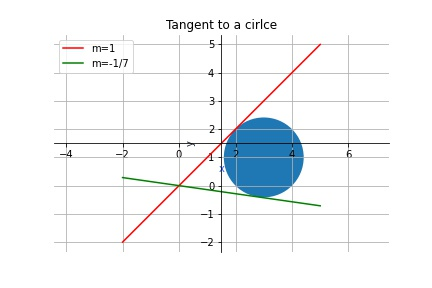
\includegraphics[width=1\columnwidth]{tangent.jpg}
\caption{Circle with tangent}
\end{figure}


\end{document}